%Dette er utf8x udgaven af LaTeX-templaten. Den er til brug på systemer der kører utf8x, såsom Linux. Hvis du bruger Windows, så er det letteste at bruge TeXmaker som editor.
% Loader dokumentklassen memoir. Sætter sproget i dokumentet til dansk, papirtypen til A4, sætter dokument til lige store højre og venstre margen, laver en søjler og siger at vi gerne vil lave en artikel, sætter skriftstørrelse til 11pt.
\documentclass[danish,a4paper,oneside,onecolumn,article,11pt]{memoir}
\usepackage[danish]{babel}		%Giver mulighed for dansk orddeling. Slet kun hvis du VED hvad du laver, eller skal skrive noget på engelsk.
\usepackage[utf8x]{inputenc}	%Her sættes tegnsæt til utf8x.
\usepackage{graphicx}		%Tillader indsættelse af billeder
\usepackage{mathtools}		%Ekstra matematik... bare lad den være, du får muligvis brug for den.
%\usepackage{url}		 %bruges til at formattere url'er... kan sagtens udelades.
\usepackage[colorlinks=true]{hyperref}
\usepackage[draft]{fixme} % Denne pakke tillader indsættelse af fixme noter ved brug af \fxnote{} som man kan bruge som huske sedler til sig selv.

\usepackage{listings} % Hvis man vil inkludere kode eksempler.
\lstset{language=matlab,breaklines=True} % Indstiller syntaks highlight til Matlab.

% Caption styles: Laver alle captions om til sans serif fonte og gør dem en smule mindre end brødteksten.
\captionnamefont{\small\sffamily}
\captiontitlefont{\small\sffamily}


\usepackage{soul} % lege lege -- Dette er til forsiden
\sodef\an{}{0.2em}{.9em plus.6em}{1em plus.1em minus.1em}
\newcommand\stext[1]{\an{\scshape#1}}



\usepackage{microtype} % Pakke der proever at fikse badbox problemer. Kun kompatibel med pdflatex.
% For at indstille margin:
%	   		         left   right ratio
\setlrmarginsandblock{2cm}{2cm}{*} % Hvor stjerne betyder udfyldes "automatisk".
%                     top    bot ratio
\setulmarginsandblock{2cm}{2cm}{*} % Hvor stjerne betyder udfyldes "automatisk".
%\setlength{\oddsidemargin}{0cm} %giver mere plads på siden
\checkandfixthelayout

\pagestyle{simple} %Giver tom footer og sidetal i header




\begin{document}
%Her laver vi en flot forside...
\begin{titlingpage}
\thispagestyle{empty}
\centering
{ \setlength{\baselineskip}{24pt}
{\Huge \stext{Kvantemekanikprojekt  Q1+Q2, 2017}} \par\vspace*{2\onelineskip}

%%%%% HUSK AT ÆNDRE TITEL HER %%%%%%%%%%%%
\large\stext{Projekt nr: X} \par %<--- I stedet for X skriver du nr. på jeres projekt%%%%% HUSK AT ÆNDRE X HER %%%%%%%%%%%%
\large\stext{Titel: ZXY GHF GT} %<--- Her skriver du titlen på jeres projekt%%%%% HUSK AT ÆNDRE TITEL HER %%%%%%%%%%%%
%%%%%%%%%%%%%%%%%%%%%%%%%%%%%%%%%%%%%%%%%%
\par\vspace
*
{8\onelineskip} %Her skrives dit navn og dit årskortnummer
\large\stext{Navn: XX YY} \par
\large\stext{Studienummer:  123456789}\par\vspace*{2\onelineskip}
%% Skal flere gruppemedlemmer tilføjes, så kopier ovennstående to linjer, eller udkommenter og kopier nedenstående tre linjer ved individuel besvarelse.

%\large\stext{Projektet er udf\o rt i samarbejde med:} \par
%\large\stext{Navn: XX2 YY2 } \par
%\large\stext{{\AA}rskortnummer:  123456789}\par\vspace*{2\onelineskip}

\large\stext{Vi afleverer en f\ae lles besvarelse - individuelle besvarelser (ret til det korrekte) }\par\vspace*{2\onelineskip}
\large\stext{Afleveret: dato (Senest 8/12 kl.~12.00 til Ann-Berit Porse
St\ae rk\ae r, 1520-629) }\par\vspace*{2\onelineskip}
}
\vfill
\vspace
*
{2\onelineskip}
%%%% HER SKAL I SKRIVE VEJLEDEREN PÅ PROJEKT OG JERES TØ-INSTRUKTOR %%%%
%%%% HVIS I HAR FORSKELLIGE INSTRKTORE TIL TØ, SÅ SKRIV DEM ALLE %%%%%%%
\stext{Projektvejleder: XXX YYY}\par\vspace*{2\onelineskip}
\stext{Instruktor: XXA YYA}\par\vspace
*
{2\onelineskip}
\enlargethispage{2\onelineskip}
\end{titlingpage}



\chapter{Indledning}
Formålet med projektrapporten er at forklare projektets formål,
metoder og resultater for en læser, som har fulgt kvantemekanik, men
ikke nødvendigvis kender til detaljer i emnet, I har studeret. Det er
derfor vigtigt at rapporten er skrevet i et klart og \emph{korrekt}
sprog. Studieordningen for fysik skriver specifikt,

\begin{quote}
  "Ved bedømmelsen af bachelorprojekt, kandidatspeciale, masterprojekt
  og andre større skriftlige opgaver skal der ud over det faglige
  indhold også lægges vægt på den studerendes stave- og
  formuleringsevne."  \sourceatright{{Studie-ordning for
      bachelorudd. i fysik (2015) \cite{studieordning},}}
\end{quote}
og i læringsmålene for kvantemekanik står der at I skal
\begin{quote}
  "Gennemføre og afrapportere et projektforløb - under vejledning af
  lærer - inden for et kvantemekanisk emneområde, inklusive
  litteraturstudier, beregninger samt selvstændig formulering af en
  skriftlig rapport over emnet."  \sourceatright{{Kursusbeskrivelse
      for kurset Kvantemekanik (E2017).}}
\end{quote}


Nedenfor følger eksempler på hvordan formler kan skrives ind, hvordan
figurer kan sættes op samt hvordan henvisninger/referencer angives i
teksten. Husk at nummerere formler, der henvises til.  Ønskes
rapporten skrevet i Word, så skal I designe jeres rapport så I får
samme layout som denne, både i forhold til marginer, skrifttype,
formler, referencer osv. Marginer er sat til 2 cm (højre/venstre) og 2
cm (top/bund) og der er skrevet med serif-skrifttype (f.eks. Times New
Roman) med størrelse 11pt. Forsiden og litteraturlisten tæller ikke
med i jeres 6 sider.

Til sidst: \emph{Husk} at læse jeres rapport omhyggeligt igennem for
trykfejl inden I afleverer.

\begin{figure}
\begin{center}
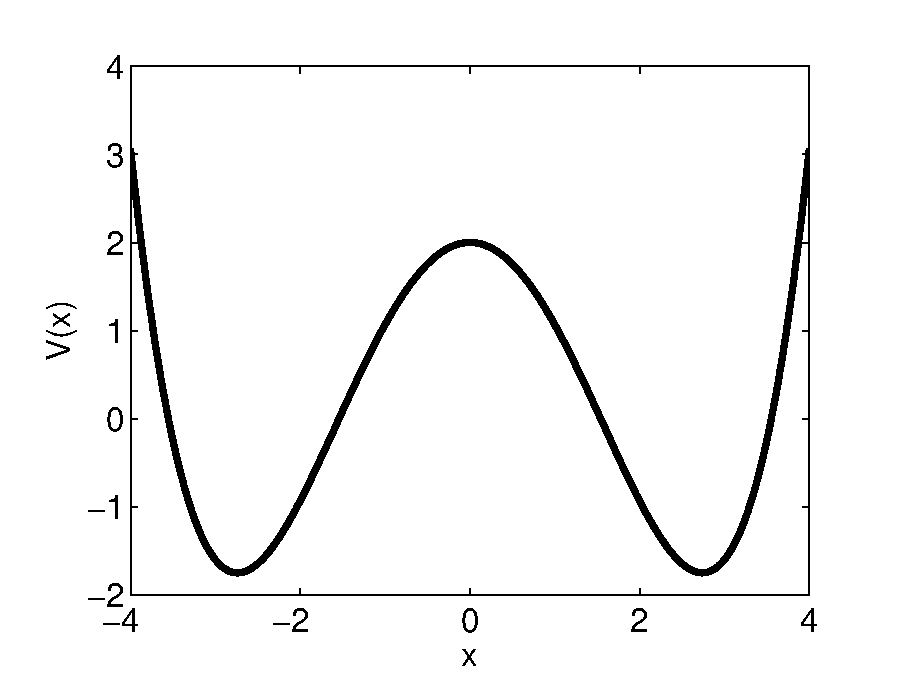
\includegraphics[width=0.5\columnwidth]{potential.eps}
\caption{Her ses et potentiale. Brug denne kommando når I skal
  indsætte figurer. Det er ikke så vigtigt hvor figurer er placeret,
  så længe det er i nærheden af der, hvor I henviser til figuren.}
\label{fig:pot}
\end{center}
\end{figure}

\chapter{Eksempel på Udregninger}
\section{Indledning}

% \section{Solution to the stationary Schrödinger Equation}
Antages, at der betragtes en partikel i en dimension, $x$,  er Schrödinger ligningen
\begin{equation}
    \frac{\hbar^2}{2m}\frac{\partial^2 \psi}{\partial x^2} + V(x) \psi = E \psi
    \label{eq:scrodingerLigning1}
\end{equation}
isoleres $\frac{\partial^2 \psi}{\partial x^2}$ i \cref{eq:scrodingerLigning1}, opnås
\begin{equation}
    \frac{\partial^2 \psi}{\partial x^2} = 2m\psi (E  - V(x)) \frac{1}{\hbar^2}
    \label{eq:scrodingerLigning2}
\end{equation}
defineres $p(x)$ klassisk
\begin{equation}
p(x) \equiv \sqrt{2m(E-V(x))}
\end{equation}
Kan \cref{eq:scrodingerLigning2} omskrives til
\begin{equation}
    \frac{\partial^2 \psi}{\partial x^2} = - \frac{p^2}{\hbar^2} \psi.
    \label{eq:scrodingerLigning3}
\end{equation}
Anvendes ansatzen
\begin{equation}
    \psi(x) = A(x) e^{i \phi(x)}
    \label{eq:ansatz}
\end{equation}
hvor $\psi (x)$ e$ \in \mathbb{C}$. Antages
\begin{equation}
 E > V(x) \forall x
\end{equation}
Er $A(x)$ en reel amplitude og $\phi(x)$ er en reel fase. Dette kan altid gøres, der man ved hjælp af ledet  $e^{i \phi(x)} $. Dette led danner en vektor $ \in \mathbb{C}$ med normen 1, herefter kan $A(x)$  skalere vektoren, til at ramme alle punkter. Anvendes venstre side af \cref{eq:scrodingerLigning3} på \cref{eq:ansatz} fås (hvor mærke $'$ angiver differentation med hensyn til x)
\begin{equation}
    \frac{\partial \psi}{\partial x} = e^{i \phi(x)}(A' + iA\phi ')
    \label{eq:diff1gange}
\end{equation}

\begin{equation}
    \frac{\partial^2 \psi}{\partial x^2} =
    \label{eq:diff2gange}
\end{equation}

% \section{kvantisering}
Vi antager nu at vi har det klassiske vendepunkt, hvor $E > V(x) $ for alle $ x$. Vi siger nu at vores bølgefunktion kun må eksistere på x-intervallet [a,b], hvilket medfører at vores sandsynlighedstæthed skal være 0 udenfor dette interval, altså $|\psi|^2 = 0$. Dette medfører at $\psi = 0$
Ser vi på bølgefunktionen, $\Psi$, ser vi at vi kan skrive den som to dele:
\begin{equation}
  \psi(x) \cong \frac{1}{\sqrt{p(x)}}\left[C_1e^{i\phi(x)}+C_2e^{-i\phi(x)}\right]
  \label{eq: kvantiseringStart}
\end{equation}
Her ses det at vi kan skrive dette om, ved at definere to nye konstanter, $C_3 \equiv i(C_1-C_2)$ og $C_4 \equiv C_1+C_2$.
\begin{equation}
  \psi(x) = \frac{1}{\sqrt{p(x)}}
  \Bigl[    C_3\sin{\phi(x)}+C_4\cos{\phi(x)}   \Bigr]
  \label{eq: kvantiseringSinCos}
\end{equation}

% \section{The Hydrogen Atom}
Schrödingerligningen skrives

\begin{equation}
    \frac{-\hbar}{2m}\diff
    \label{<+label+>}
\end{equation}<++>


% \section{Solution to the stationary Schrödinger Equation}

% \section{Ionisation af et Rydberg-atom}

% \section{Konklusion}
I denne rapport undersøges WKB approksimationen. Først udledes approksimationen fra Schrödingerligningen, i én dimension. Vi finder en løsning der bygger på at $V(x)$ varierer langsomt, i forhold til bølgelængden af $\psi(x)$, og dermed forventer at et mere konstant potentiale giver et bedre svar. Eksempelvis finder vi, at approksimationen faktisk levere et eksakt svar, til de tilladte energier for et uendeligt brøndpotentiale. Dernæst undersøges brintatomet. Vi finder at energiernes løsninger afhænger af kvantetallet $l$, og at WKB-approksimationen giver bedre resultater, når det gælder at $n'$ er meget større end $l$. Det ved vi, da vi netop kan løse energierne for brint eksakt. Afslutningsvist undersøges den asymptotiske form for bølgefunktionerne for brint hvor det findes at approksimationen går imod de eksakte løsninger for store radier $r$.


\begin{thebibliography}{99}
\bibitem{studieordning} \href{https://mit.au.dk/EDDI/webservices/DokOrdningService.cfc?method=visGodkendtOrdning&dokOrdningId=10727&sprog=da}{Studieordning for bacheloruddannelsen i fysik
  (2015)}.
\bibitem{griff} Introduction to Quantum Mechanics, Second Edition, David J Griffiths.
\bibitem{schaums} Schaums's Mathematical Handbook of formulas and Tables, Third Edition, Murray R Spiegel et.~al.
\end{thebibliography}

\end{document}
